\documentclass[a4paper,12pt]{article}
\usepackage{graphicx}
\usepackage{longtable}
\usepackage{rotating}  % for sideways table
\usepackage[utf8]{inputenc} % Required for inputting international characters
\usepackage[T1]{fontenc} % Output font encoding for international characters
%\usepackage{fancyhdr} % Load the fancyhdr package
\usepackage[margin=1in]{geometry} % Optional, to control page margins
\usepackage{xcolor} % to determine colors
\usepackage[
    backend=biber,
    maxnames=2,
    style=authoryear,
    date=year]{biblatex} % Use the bibtex backend with the authoryear citation style (which resembles APA)
\usepackage{hyperref}
\hypersetup{colorlinks,
citecolor=teal,
linkcolor=cyan,
urlcolor=olive
}

% load references
\addbibresource{ms_crete_soil.bib}
% Adjust bibliography font size
\renewcommand*{\bibfont}{\small} % Use \footnotesize, \small, or other sizes
% title
\title{Harnessing Heterogeneous Data for Soil Health Assessment in Island Landscapes}
% authors
\author{
Savvas Paragkamian\textsuperscript{1,2,\dag, *},
Johanna B. Holm\textsuperscript{3\dag},
Haris Zafeiropoulos\textsuperscript{4}, \and
Christina Pavloudi\textsuperscript{5},
Christos A. Christakis\textsuperscript{1}, \and
Ioannis Antoniou\textsuperscript{8},
Panagiotis F. Sarris\textsuperscript{1,8}, \and
Lynn Schriml\textsuperscript{3},
Giorgos Kotoulas\textsuperscript{2, \ddag, *},
Evangelos Pafilis\textsuperscript{2, \ddag, *}
}
\begin{document}

\maketitle

\begin{center}
\textsuperscript{1} Department of Biology, University of Crete, Voutes, 70013, Crete, Greece \\
\textsuperscript{2} Institute of Marine Biology, Biotechnology and Aquaculture (IMBBC), Hellenic Centre for Marine Research (HCMR), Gournes, 71500, Crete, Greece \\
\textsuperscript{3} University of Maryland School of Medicine, Institute for Genome Sciences \\
\textsuperscript{4} Department of Microbiology, Immunology and Transplantation, Rega Institute for Medical Research, KU Leuven, Leuven, Belgium \\
\textsuperscript{5} European Marine Biological Resource Centre, Paris, France \\
\textsuperscript{6} Department of Mathematics, Aristotle University of Thessaloniki, 54124, Thessaloniki, Greece \\
\textsuperscript{7} Department of Environmental Science and Technology, University of Maryland, Baltimore, USA \\
\textsuperscript{8} Institute of Molecular Biology and Biotechnology, Foundation for Research and Technology-Hellas, 714 09 Heraklion, Crete, Greece
\end{center}
\vspace{1em}

\noindent\textsuperscript{\dag} These authors contributed equally as first authors. \\
\noindent\textsuperscript{\ddag} These authors share last authorship. \\
\noindent\textsuperscript{*} Corresponding authors: \texttt{s.paragkamian@hcmr.gr}, \texttt{kotoulas@hcmr.gr}, \texttt{pafilis@hcmr.gr}

\begin{abstract}

    A synthesized knowledge base of microbial biodiversity, in terms of
    ecological and remote-sensing data remains a major challenge.
    Many worldwide studies have been published regarding soil
    microbiome ecosystems, though there are still many blind spots.
    Islands can be important case studies for this integration for more resolute and dense samplings.
    Here, we utilize the Island Sampling Day Crete 2016 microbial 16S rRNA gene
    amplicon data, integrated with soil and remote
    sensing data, to decipher the drivers of ecosystem function of the island.
    The Island Sampling Day Crete 2016 project has collected 144 topsoil samples
    from 72 sites, capturing a lot of this diversity, accompanied by FAIR
    (Findable, Accessible, Interoperable and Reproducible) data by design. 
    Cretan macroecology has been studied for centuries for its diverse  and endemic
    fauna and flora.
    In addition, Crete has been considered as a miniature continent with high contrasts in
    vegetation cover, elevation, climatic conditions. 
    We show that, higher altitudes in Crete found to
    be inhabited by a more diverse number of microorganisms, a pattern commonly
    seen in several faunistic groups, such as arthropods.
    The integration of the spatial data with state of the art methods enabled warning signals
    in pristine and grazing ecosystems.
    These results along with the
    climatic and desertification index influences on the soil microbiome of Crete,
    provide the basis to identify major drivers of biodiversity, to evaluate hotspots
    and contribute to foreknowledge of threatened ecosystems.

\end{abstract}

\noindent\textbf{Keywords:} soil microbiome, networks, island, Crete, spatial data, remote sensing, data integration, FAIR data\\

\noindent\textbf{Highlights}

\begin{itemize}
    \item Towards a data soil scape of an island
    \item Building a system based on the rich open data about Crete island allows for complex associations and novel hypotheses
    \item There is wealth of data about Crete in many different forms and databases across ecosystem scales and scientific disciplines,
    \item Data integration of soil in Crete revealed vulnerable ecosystems
\end{itemize}


\section{Introduction}\label{intro_idea}

Disentangling the soil ecosystem functioning requires an holistic and 
multidisciplinary approach \parencite{vogel2022}. 
Soils are characterised by multiple properties; chemical (pH, nutrients etc.),
physical (grain size, clay content etc.) and biological that 
form complex interdependent interactions \parencite{philippot2024the-interplay}.
Biodiversity of soils covers
all forms of life, fauna, flora, bacteria, archaea, fungi, viruses \parencite{Orgiazzi2018,Anthony2023}. 
Bacteria and archaea are considered major drivers for the functionality of soil.
They influence and are influenced by their environment and their community structure 
defies their macroscopic functionality \parencite{Bahram2018}.

Global soil microbiome studies have been employed to decipher microbial community
compositions \parencite{fierer2012cross-biome,thompson2017a-communal, Delgado-Baquerizo2018, Labouyrie2023},
functions \parencite{Bahram2018} and biogeography \parencite{Martiny2006, Guerra2020}.
The integration of the these multifaceted 
data is needed to decipher and control soil functioning \parencite{ramirez2015toward}.
All this work is needed in order to meet
UN and EU soil goals for the 2030 and 2050 for healthy soils \parencite{LAL2021e00398}.

Data and metadata of these samplings are stored in databases towards
a global effort to enable Findable Accessible Interoperable and Reusable (FAIR) data \parencite{Wilkinson2016}.
For sequencing data the Genomic Standards
Consortium (GSC) \parencite{Field2011} has established checklists, like the MIMARKS \parencite{yilmaz2011minimum}
standards among others, and has been an advocate for open and unrestricted data \parencite{Amann2019}.
There are global resources and platforms databases like ENA \parencite{ocathail2024the-european},
JGI Genome Portal \parencite{nordbergGenomePortalDepartment2014a} and others.
Biodiversity is represented in ecosystems as point occurrences of each taxon. The
DarwinCore standards have enabled global of species occurrences \parencite{Wieczorek2012}.
GBIF is a global aggregator that contains such information about all ecosystems from 
different resources \parencite{noauthor_gbif_nodate}. 
IUCN redlist \parencite{iucn2024} is also an important resource of species occurrences,
habitats, threats and conservation status of taxa. Redlists contain 
manually curated content by experts of each taxonomic group which is updated
after some years depending on the country and group.

Open data soil data are are hosted by the 
European Soil Data Centre \parencite{panagos2022european}, edaphobase 2 \parencite{russell2024edaphobase}
and the World Soil Information Service (WoSIS) of the ISRIC \parencite{Batjes2024}. Regarding the latter, a unified
platforms called SoilGrids provides open access to many predicted maps \parencite{poggio-soil-7-217-2021}.
Apart from samplings,
spatial and remote sensing data are openly available terrestrial ecosystems.
To name a few, there openly available climatic \parencite{Fick2017}, land cover change \parencite{winkler2021global} and normalized
vegetation index \parencite{CopernicusNDVI2021}.
There is also a wealth of knowledge about soil and biodiversity in the literature,
albeit in unstructured format. 
Databases like PubMed MEDLINE \parencite{sayers2024database}, Google Scholar, Dimensions and Biodiversity Heritage Library 
are world class providers with different content.

The heterogeneous data those presented above are the basis of investigating the
interactions of organisms with their surroundings through systems ecology \parencite{van-dyne1966ecosystems}.
The representation of ecosystems with data was first mentioned as "digital earth" in the late 90s \parencite{Goodchild_2012}.
This notion of the virtual earth was initially realised with satellite imaging,
on-land sensors and the relevant software. Space, an area on Earth, is
the starting point of ecosystems functioning which is influenced by geography,
climate, geology, biodiversity and human management across scales \parencite{Zarnetske2019_towards}.
The coupling of all these
fields, and the data they provide, with spatial information leads to the
digital twin of ecosystems \parencite{Voosen2020DigitalTwinEarth}. All these data can be considered as different layers
of an Earth system data cube \parencite{mahecha2020earth}.

The global and continental studies discovered the remarkable diversity in soils yet there are blind spots \parencite{Guerra2020}.
Most soil samplings are sparse when considering the scale and the samples per area density \parencite{Dini-Andreote2021},
apart from selected studies e.g \textcite{Karimi2020}.
To tackle this challenge there have been established model systems and scientific stations such
as the Middle east natural laboratory \parencite{blanco-sacristan2024the-middle}.

"Scapes" are a promising approach towards the digital earth due to their smaller 
scale and scope.
Landscape scale, and not global or regional, has been deemed as crucial for monitoring and assessing 
Soil Organic Carbon dynamics \parencite{doetterl2025a-landscape-scale}.
In addition, the joining of the natural and human activities 
together has been defined in the so-called soilscape \parencite{LAGACHERIE2001105}.
Regarding heterogeneous data, datascape framework is promising for data explorations of soil information \parencite{rolland2024datascape:}. 
Islandscapes 
is also an interesting approach which defines the holistic ecosystem of the island
and the interface of land and sea \parencite{Vogiatzakis_land_2017}.

Islands due to their smaller scale and confined nature are useful virtual ecological labs.
They harbour 20\% of biodiversity even though they cover less than 7\% of land surface area.
Also they are under major threats that diminish their biodiversity \parencite{fernandez-palacios2021scientists}.
Important examples are the work of \textcite{Li2020} on soil bacteria and of \textcite{Delavaux2021} on mycorrhizal fungi studies
in islands which show the benefits of using islands as models.
The Island Digital Ecosystem Avatar (IDEA) is a digital representation of Mo'orea island,
French Polynesia that has managed to integrate satellite data with sequences,
bringing together all scales of biodiversity \parencite{Davies2016,davies2023island}.

The island of Crete, Greece is a continental forarc island \parencite{ali2016},
fifth largest island of the mediterranean (8350 km\textsuperscript{2}),
and a mediterranean biodiversity hotspot \parencite{myers2000biodiversity}.
It has been studied since the classical times for its'
fauna \parencite{Sidiropoulos_Polymeni_Legakis_2017,Anastasiou2018Tenebrionid},
flora \parencite{Krimbas_2005} and ecosystems \parencite{Grove1993}.
It is home to the only endemic mammal of Greece, the Cretan shrew (\textit{Crocidura zimmermanni}),
more than 350 endemic arthropods \parencite{bolanakis2024} and 183 endemic plants \parencite{Kougioumoutzis2020}
among them a tree \textit{Zelkova abelicea}.

Crete has been characterised as a miniature continent \parencite{Vogiatzakis2008_crete} because 
of it's diversity of landscapes and seascapes.
Multifaceted factors have shaped the
biodiversity of the island, for example the sharp elevation gradient \parencite{trigas2013, FAZAN2017},
the complex evolutionary history \parencite{POULAKAKIS2002} and the human - nature
interactions over thousands of years \parencite{Vogiatzakis2008_med, Sfenthourakis2017}.
The major threats of human activities are becoming apparent in the island's ecosystems,
like desertification \parencite{KARAMESOUTI2018266}, soil erosion \parencite{panagos2014seasonal}, intensive grazing \parencite{JouffroyBapicot2016},
climate change \parencite{Kougioumoutzis2020,Vogiatzakis2016} and habitat loss \parencite{ISPIKOUDIS1993259}.
The soil microbiome has been studied in protected areas,
i.e Natura2000 \parencite{bekris2019do-genetic}, and across the islands' ecosystems \parencite{holm2025first}.
All these data are further establishing Crete as a great soil model island.

In this study we ask: which are the resources of open data regarding soil ecosystems of Crete?
How can we integrate these data to investigate the functioning of soil?
Are there any alarming soil health signals in Crete derived from this integration?
To address these questions, first we create a data repository categorised in 
literature (text), samplings (point data) and spatial data (maps). 
We proceed to summarise each resource contents and
identified gaps and opportunities for subsequent analyses.
Our aim is to establish a FAIR data summary of Crete in order to enable integrative analyses.
To further support our case we use the
Island Sampling Day (ISD) soil microbiome data \parencite{holm2025first},
as a large scale bacterial study, to gain insights about the differences of the
microbiome communities across land use, aridity and functional categories in Crete island.

\section{Materials and Methods}\label{integration_methods}

Multiple resources and types of data are required to create
a Cretan soil biodiversity data system (Figure \ref{fig:crete_idea_fig1}). 
First, data were categorised in literature, sampling data (biodiversity occurrences and soil samples)
and maps (spatial layers or rasters and vectors).
Then, resources with open data about Crete were identified and retrieved in each category.

\begin{figure}[hbt!] 
    \centering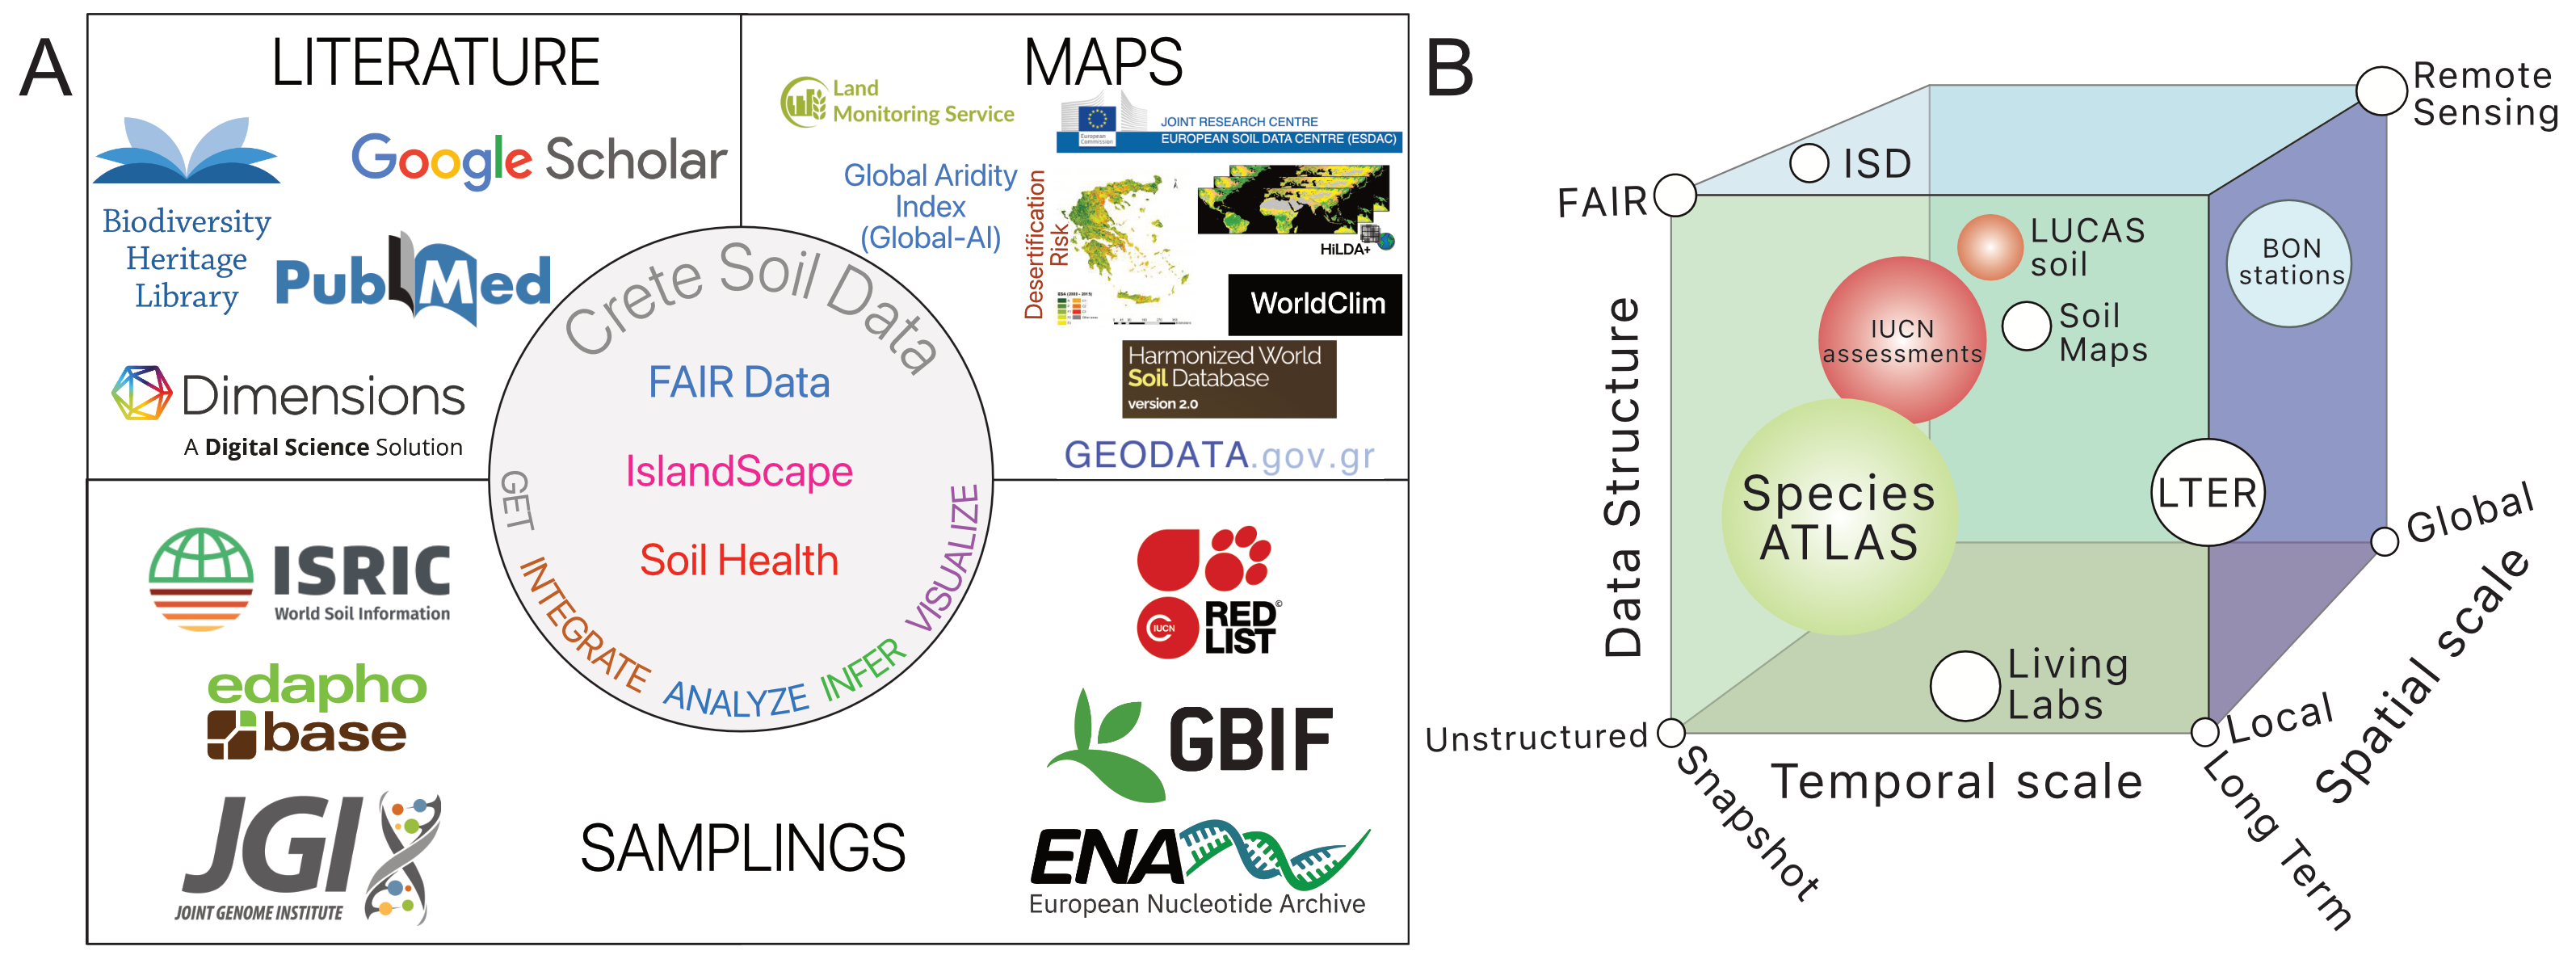
\includegraphics[width=\columnwidth]{figures/crete_idea_fig1.png}
    \caption{A. Resources that contain data about Crete categorized in Literature, Maps and Samplings. B. Data derived from A are placed in the ecological data space with according to the Spatial scale, Temporal scale and Data structure.}
    \label{fig:crete_idea_fig1}
\end{figure}

\subsection{Literature}\label{crete-literature}

The name of Crete is unambiguous word which reduces the false positives when performing queries in databases.
Searches were done using different mentions of Crete such as \textit{Crete, Kriti, Kreta, and Cretan} in PubMed MEDLINE, 
Google Scholar, Dimensions and Biodiversity Heritage Library.
First, the MEDLINE PubMed corpus was downloaded via the ftp protocol and the E-utilities API.
After XML files processing, the following fields were kept: PMID, DOI, Authors, Journal, Volume:Pages, Year, Title, Abstract.
Pubmed was searched using the DIG tool \parencite{fanini2021coupling}.
Each abstract of MEDLINE contains also associated MeSH terms which were retrieved with the \href{https://www.ncbi.nlm.nih.gov/books/NBK25497/}{E-utilities API}
and were later summarised with custom scripts.

The Dimensions platform provides a web service for complex queries 
which was used to identify literature of 
\textit{Crete, Kriti, Kreta, and Cretan} within
the title and abstract fields. Output also contained the Field of Research of 
each bibliographic entry.
Google scholar was used through the \textit{serpapi} API using
a python script. The same keywords were used as in the previous searches.

Historical literature related to the biodiversity of Crete has been explored
using the Biodiversity Heritage Library (BHL) data model and schema, conducting searches on titles, items, and subjects.
Items represent the digitised documents, while subjects are assigned to each title.
The schema includes a page table with page-level information.
An archive of all transcribed texts was downloaded and search was performed on each page 
and subject.

\subsection{Samplings}\label{crete_samplings}

The data of samplings contain sequences (fastq files), biodiversity occurrences (tab separated files)
and soil (tab separated files), using ENA, GBIF and WoSIS respectively.
The ENA API was used with a POST request containing the bounding box of Crete as a query \parencite{yuan2023the-european}. This 
query returned a list with the sample identifiers. Using this list and a custom python script the API
was invoked with GET requests to retrieve all the available metadata for each sample.
The GBIF online user interface was used to query occurrence data contained in
the bounding box of Crete \parencite{noauthor_gbif_nodate, gbif.org-user2023occurrence}.
IUCN redlist point data and summary of assessments were downloaded from the web interface \parencite{iucn2024}.
Advanced filters were selected, for Land Regions option \textit{Kriti} was opted
along with Global, European and Mediterranean scopes.
WoSIS soil data and metadata about Crete were retrieved using the Web Feature Service (WFS) \parencite{Batjes2024}
along with an adjusted R script.
Edaphobase, a curated database of museum records, was also searched for soil biodiversity \parencite{BURKHARDT20143}.

\subsection{Maps}\label{crete_spatial}

Maps that were build for Crete or broader maps, e.g global,
were downloaded and cropped from multiple resources.
The land use categories were obtained from the CORINE Land Cover (CLC) 2018
version v.2020.20u1 \parencite{CLC2023}.
The Historic Land Dynamics Assessment (HILDA+) dataset \parencite{winkler2021global}
facilitated the exploration of human pressures, such as changes in land usage and agriculture,
allowing the calculation of land use alterations from 1998 to 2018.
The protected areas of Crete were included as well from the World Database on Protected Areas using the wdpar package \parencite{Hanson2022}.
In WorldClim 2.0, with climatic variables, such as the annual mean
temperature and annual precipitation, were included \parencite{Fick2017}.
The dataset on the Environmentally Sensitive Areas Index to desertification (ESAI)
in Greece \parencite{KARAMESOUTI2018266} was also employed, alongside the
Global Aridity Index Database \parencite{zomer2022version}.
The geological formations of Crete were derived from the geoportal of the
Decentralized Administration of Crete. These maps were created by the Crinno-Emeric Group
project \url{https://geoportal.apdkritis.gov.gr/gis/apps/storymaps/stories/19690f65abbe4e8ab0141b2fe7261a8c}.
Furthermore, the Harmonised World Soil Database v2 was integrated for soil
mapping units and taxonomic soil classification \parencite{fao2023}.

\subsection{Health assessments of Island Sampling Day Crete}\label{isd_data}

This study uses the ISD Crete data that have been deposited
in the European Nucleotide Archive (ENA) at EMBL-EBI under accession number PRJEB21776.
The raw sequences (fastq files) and metadata (xml files) were downloaded with custom scripts using the ENA API \parencite{Yuan2023}.
Specific information regarding the ISD sampling, DNA extractions, PCR and sequencing
protocols are discussed here \parencite{holm2025first}.

Amplicon Sequence Variants were inferred using DADA2 \parencite{Callahan2016} for 
filtering, denoising and chimeric reads removal. Normalisation of the reads at 10000 reads
across samples was implemented with the SRS R package \parencite{Beule2020}. Samples
with less than 10000 reads were removed. ASVs were assigned to taxonomy using 
DADA2 with Silva 138 taxonomy \parencite{quast_silva_2013}.
PEMA was used for OTU inference based on VSEARCH \parencite{zafeiropoulos2020pema} with Silva 132 taxonomy.

The numerical ecology analyses, e.g diversity indices, NMDS, PERMANOVA, were calculated
with the vegan R package \parencite{oksanen2024vegan}.
For PCoA ordination the ape R package \parencite{Paradis2004} and UMAP python library \parencite{mcinnes2018umap-software}.
U-CIE R package was used for coloring 3 dimensional data \parencite{Koutrouli2022} to 
visualise the $\beta$ diversity differences of samples on the map.
Taxa functional annotation was implemented with the manually curated FAPROTAX database
with the accompanied python script \parencite{Louca2016}.
%The network inference was facilitated with FlashWeave 0.19.2 \parencite{Tackmann2019}.
%To use FlashWeave we reduced 
%the abundance table of the ASVs to keep the ones at the genus or species level.
%The subsequent network analyses were carried out
%with the igraph R package \parencite{Csardi2006}. 
The differential abundance analysis was facilitated with the ANCOM-BC2 R package \parencite{Lin2023} using the 
different spatial layers from the maps section.

\subsection{Tools and code}\label{Coding environment}
The working environment had Python 3.11.4, R version 4.3.2 \parencite{rcoreteam}.
In terms of managing spatial data, geometry, and transformations, the following
R packages were used:
sf package version 1.0-14 \parencite{Pebesma2023}, for polygons, and the terra
package version 1.7-55 \parencite{hijmans2024terra}, for rasters.
Visualisation was implemented with ggplot2 \parencite{wickham_ggplot2_2016} and pheatmap \parencite{Kolde2019}.
Taxon names resolve and taxonomic classification was facilitated by taxize R package \parencite{chamberlain_taxize_2013}.
Finally, computations were performed on HPC infrastructure of HCMR \parencite{zafeiropoulos_0s_2021}.
Scripts about data integration are available in
\href{https://github.com/savvas-paragkamian/crete-idea.git}{Crete data integration repository}.
Scripts about the soil health assessment are available in 
\href{https://github.com/savvas-paragkamian/crete-soil-health.git}{Crete soil health assessment repository}.

\section{Results and Discussion}\label{crete_idea_results_discussion}

The collection of different data types for one island, Crete, required the investigation
of a multitude of resources with distinct information, Figure \ref{fig:crete_idea_fig1}A.
These data are open access
yet their integration and interoperability requires manual effort and curation. 
Bringing all these data together allowed for a schematic representation regarding their
data structure, temporal scale and spatial scale, represented in Figure \ref{fig:crete_idea_fig1}B. 
For example, species biodiversity occurrences (Atlases), e.g Atlas of the Hellenic flora \parencite{strid2024atlas}, 
are monumental works, albeit lacking structured data standards and they are 
limited in their temporal scale. Whereas, Remote Sensing data follow global 
standards, cover the globe and also produce time series data.
Biodiversity Observation Networks (BON stations) are available only for marine systems
currently, e.g. ARMS \parencite{obst2020arms,santi2023emobon}, 
which provide long term monitoring samples, in a regional scale while aiming at 
high quality metadata and standards. 
Living Labs \parencite{alhajj-ali2025a-review}, are also an novel approach focusing on 
monitoring agriculture in the local scale, they haven't focused on 
the adoption of standards and FAIR data.

%data cubes and the species occurrences cube \parencite{oldoni2020occurrence,groom2023b-cubed:}

\subsection{Literature}

Contemporary literature material is indexed in different platforms \parencite{harzing2019two-new-kids, walters2025comparing}
Regarding Crete, PubMed custom search resulted in 1556 unique abstracts. 
The Google Scholar API returned 910 documents and the Web service of Dimensions 
displayed an impressive 43.000 publications. 
Each platform has a different way to interact and most importantly contained 
material from subject fields about Crete, as shown in Table \ref{table:crete_literature}.

\begin{table}[htbp]
\centering
\caption{Document items about Crete and their top 6 categories across PubMed, Dimensions, and Google Scholar. The list is not exhaustive and some documents can be in multiple categories}
\label{table:crete_literature}
\begin{tabular}{|p{2.5cm}|p{2.5cm}|p{2.5cm}|p{2.5cm}|p{2.5cm}|p{2.5cm}|}
\hline
\textbf{PubMed MeSH terms} & \textbf{PubMed abstracts} &
\textbf{Dimensions Fields of Research} & \textbf{Dimensions} &
\textbf{Google Scholar categories} & \textbf{Google Scholar} \\
\hline
Human & 907 & History, Heritage, Archaeology & 2834 & Biodiversity & 228 \\
\hline
Genetic phenomena & 500 & Earth sciences & 2284 & History & 200 \\
\hline
Behaviour Mechanisms & 500 & Education & 2822 & Archaeology & 191 \\
\hline
Infections & 200 & Historical studies & 1925 & Sociology & 136 \\
\hline
Organic chemicals & 200 & Biomedical and Clinical Sciences & 1463 & Folklore & 118 \\
\hline
Environmental sciences & 177 & Language, Communication and Culture & 1490 & Other & 37 \\
\hline
\end{tabular}
\end{table}

Regarding the historical literature from BHL,
The largest biodiversity library is BHL with 62 million text pages from 292,000 unique documents. 
All pages were searched to find the documents relevant of Crete which resulted in
3,696 documents and 35,130 pages exhibited five or more occurrences of keywords related to Crete.
Taxon named recognition based on the gnfinder tool on each OCRed page of BHL \parencite{mozzherin_gnamesgnfinder_2022},
revealed that 890 documents, contained more that 50 different taxon names.
Also, 1,879 items had titles in 18 languages, with the
majority being English (1,350), German (268), French (105) and others. 
The oldest publication in BHL that mentions Crete was printed in 1554 and contains
the biodiversity observations in Crete written by the famous French explorer Pierre Belon \parencite{belon1554les-obseruations}. 
In addition, there are 1482 items published before 1960 containing thousands of taxa occurrences.
Overall, the wide range of subjects in the literature, the different languages and years of historical publications illustrate the
global impact and interdisciplinary of the Cretan literature.

\subsection{Maps}

Crete is a mosaic of landscapes with diverse land cover, geology, soil type and land management,
 \parencite{Vogiatzakis2008_crete}. 
It covers an area of 8,347 km\textsuperscript{2}, encompassing contrasting features of
mountains and coastlines; gorges and plateaus; arid areas and forests; all in a confined space, Table \ref{table:crete_data_cube_area}, Figure \ref{fig:crete-data-cube-maps}.
The geology of Crete has formed through drastic tectonics \parencite{fassoulas1998the-structural} and is dominated by carbonate formations, primarily limestones
of the Tripolis (1,253 km\textsuperscript{2}), Plattenkalk (1,347 km\textsuperscript{2}),
and Pindos (248 km\textsuperscript{2}) units. 
Regarding soil type from the HWSD (Harmonized World Soil Database) reveals
Lithic Leptosols (4777 km\textsuperscript{2}) as predominant (61.11\%).
Calcaric Regosols cover about 27.82\%, and along with Lithic Leptosols 
they are frequently found on karst landscapes.

Based on the Corine Land Cover, the most common vegetation found in Crete is scrub and herbaceous (3798 km\textsuperscript{2}) 
followed by permanent crops at 2368 km\textsuperscript{2}. 
Land cover change appears to be fast the past 40 years, with shrublands being under threat,
with habitat exploitation and grazing being a major drivers \parencite{JouffroyBapicot2016}. 
The HILDA+ dataset \parencite{winkler2021global} estimates a 250 km\textsuperscript{2}
of land transitioning to urban, while 57 of urban fabric has moved to various other land types.
Cropland experienced the extensive changes, shifting 649 km\textsuperscript{2}
units to pasture/rangeland, 163 km\textsuperscript{2} to forest.

The largest part of the island is considered semi-arid (6244 km\textsuperscript{2}),
followed by dry sub-humid (1323 km\textsuperscript{2}), and humid with (537 km\textsuperscript{2}).
Desertification risk assessments reveal 1,118 km\textsuperscript{2} area
of fragile regions (F3, high fragility) \parencite{KARAMESOUTI2018266}.
Critical areas of desertification extend to 1632 km\textsuperscript{2} of low, medium and high fragility.
Erosion models of the soils of Crete showed a loss of 8.000 ha\textsuperscript{-1} year \textsuperscript{-1}
which is high for the Mediterranean, which in natural areas is attributed mostly to grazing \parencite{panagos2014seasonal}.
All these data are alarming for the loss of soil functions and desertification in Crete.
The protected areas of Crete can be used for soil conservation to counterbalance
this documented degradation. The also form networks and cover an area of 2900 km\textsuperscript{2}.
Natura2000 areas are the largest protected areas (2371 km\textsuperscript{2})
followed by the Wildlife Refuges (610.70 km\textsuperscript{2}).

\begin{figure}[!htb] 
    \centering\includegraphics[width=\columnwidth]{figures/map_crete_data_cube.png}
    \caption[Crete data cube]{The twelve layers of the terrestrial environments of Crete.
    A. The digital elevation map. B. The Corine Land Cover EEA, Level 2.
    C. The geology of Crete. D. Rivers and gorges of Crete.
    E. The Harmonised World Soil dataset, version 2.
    F. The Historic Land Dynamics Assessment dataset. G. The different protection areas of the island.
    H. The mean surface temperature of WorldClim2. I. The mean precipitation of  WorldClim2.
    J. The aridity index of soil, from the Global Aridity Index v3. K. The G2 model of soil erosion in Crete. J. The desertification risk assessment of Greece}
    \label{fig:crete-data-cube-maps}
\end{figure}


\subsection{Samplings}

\subsubsection{Biodiversity}
Open data about species occurrences in Crete discoverable through GBIF, a biodiversity aggregator.
GBIF contains 116,000 occurrences of 7065 unique species,
10189 unique taxa (Figure \ref{fig:crete-samplings}) \parencite{gbif.org-user2023occurrence}.
In total, data are provided from 196 different publishers, e.g Institutions, Museum Collections, Platforms etc.
Citizen science tools and platforms, i.e 
Cornell Lab of Ornithology, iNaturalist.org,Observation.org, Pl@ntNet and naturgucker.de,
provide the majority of data, totalling 98,571 occurrences which were excluded as non validated by experts.
The oldest occurrence is from 1684,
Historical data are also present, with 2051 occurrences and 1021 unique taxa documented 
prior to 1960 and submitted by 62 publishers, Figure \ref{fig:crete-samplings}.
Edaphobase, has in 26 resources with 17 different sampling points covering 120 distinct taxa.
A part of it is included in GBIF, yet it provides some additional functionalities. Note that 
in the center of Crete there are multiple points indicating low accuracy of locality.

IUCN redlist contains assessments from 3140 species in all geographical scopes.
Occurrences are provided for 416 species, covering 8,539 point locations, Figure \ref{fig:crete-samplings}.
Most species assessed that reside in Crete fall under Least Concern,
particularly within Tracheophyta (n = 366 Europe, 216 Global), 
Arthropoda (n = 547 Europe), and Chordata (n = 248 Europe). 
Near Threatened and Vulnerable categories occur mainly in Arthropoda and Tracheophyta.
Mollusca have higher relative counts of Vulnerable, Endangered and Critically Endangered taxa (n=23, n = 8 and n = 3, respectively).

Tracheophyta are most affected by housing and urban areas (n = 162), 
Arthropoda by Herbicides and pesticides (n = 137), 
Chordata by intentional and unintentional harvesting (n = 171), 
Mollusca and Marchantiophyta by increased fire frequency and intensity (n = 49, n = 23 respectively)
and Bryophyta by other ecosystem modifications (n = 33).
Tourism and recreation areas are attributed as major threats across phyla.
There are many important taxa of Crete not assessed yet in the aforementioned 
phyla. The newly launched IUCN Microbial Conservation Specialist Group will add microbial taxa as well \parencite{gilbert2025launching}.

\subsubsection{Monitoring}
In addition, Crete has the most long term monitoring stations in Greece, Figure \ref{fig:crete-samplings}.
Artificial reefs monitoring (ARMS-MBON) with 2 stations \parencite{obst2020arms},
European marine omics biodiversity observation network with one station \parencite{santi2023emobon},
LTER-Greece network with 3 stations \parencite{Skoulikidis2021lter} and the POSEIDON system with 2 stations \parencite{ntoumas2022}. 
These are marine (5) and terrestrial (3) station collecting biodiversity data and abiotic data.
Focusing in a confined area provides unique opportunities for data integration.
For example in Samothrace \parencite{noll2024insights} a 15 year long study 
showed practices to help sustain the socioecological system.
Crete would be a great example of the digital representation of it's ecosystems
and the human activities in order to tighten the relations with the society and 
protect vulnerable areas.

\subsubsection{Soil}
Abiotic soil data are provided by WoSIS open platform,
which contains soil taxonomy, physical and chemical metadata. 
Regarding Crete, it hosts 27 soil samples which were collected by
the Forum of European Geological Surveys (FOREGS) \parencite{nerc19017},
the Geochemical Mapping of Agricultural and Grazing Land
Soil in Europe (GEMAS) \parencite{reimann2018gemas} and the Soil Profile Analytical
Database for Europe (SPADE) \parencite{Hiederer2006}.
These data with other not publicly available,
were the basis of the \href{https://esdac.jrc.ec.europa.eu/content/soil-map-greece-0}{soil map} of Crete 
and Greece. 
Comparing the maps provided in Figure \ref{fig:crete-data-cube-maps} 
it becomes apparent that more sampling effort is required to create higher resolution maps. 

\subsubsection{Genomics and Metagenomics}
Regarding the genomic and metagenomic samples from Crete, ENA hosts all the public 
available data and metadata. There are 92 studies with 1205 samples.
From these, the 530 samples are terrestrial metagenomic samples as shown in
Figure \ref{fig:crete-samplings}. 
The most samples and studies are in the soil metagenome with 304 samples in 8 studies.
The 140 samples of which belong to the
ISD project \parencite{holm2025first}.
Insect metagenome has 108 samples from 2 studies
and plant metagenomes contains 69 samples in 2 studies.
Then follows air metagenome with 61 samples during 3 studies.

\begin{figure}[!htb] 
    \centering\includegraphics[width=\columnwidth]{figures/map_crete_samples.png}
    \caption[Samplings in Crete]{Samplings in Crete. A. GBIF occurrences in Crete.
    B. Timeline of GBIF occurrences across kingdoms. C. All genomic samples from ENA. 
    D. ENA terrestrial metagenomic samples in Crete. 
    E. Edaphobase samplings in Crete.
    F. Sampling monitoring stations in Crete include multiple LTER and BON stations.
    G. IUCN redlist data points of the assessed species in Global, European and Mediterranean scopes.
    H. WoSIS soil samples in Crete.}
    \label{fig:crete-samplings}
\end{figure}

\subsection{Soil microbiome of Crete}

The retrieval of metagenomic data revealed that multiple 
seminal worldwide soil microbiome projects include one or two topsoil
samples from Crete \parencite{Vasar2022, Labouyrie2023, Bahram2018, Orgiazzi2018}.
Some have focused on soil fungi \parencite{Mikryukov2023, Davison2021, Tedersoo2021}
and other soil eukaryotes \parencite{Aslani2022}.
The Koiliaris Critical Zone Observatory \parencite{tsiknia2014environmental}, also a LTER,
is the most thoroughly studied soil ecosystem of the island. 
Whereas the Island Sampling Day (ISD) project \parencite{holm2025first}
is the most comprehensive soil microbiome study of Crete featuring 144 soil samples 
from 72 distinct locations. 
This sampling, denser comparing continental studies with 0.017 samples per km\textsuperscript{2},
makes possible comparison across the landscapes of the island.

ISD was organised by the Genome Standards Consortium \parencite{Field2011} and the Hellenic Centre for Marine Research
as a single day event to avoid seasonality effects and to create a snapshot of soil microbiome.
ISD is an amplicon 16s rRNA marker gene study with published open data with immediate release at PRJEB21776 ENA project,
alongside rich metadata (location coordinates, DNA concentration,
total nitrogen, total nitrogen, water content, total organic carbon) \parencite{holm2025first}.

\subsubsection{Inference and taxonomy}

All available ISD sequences and metadata were downloaded from ENA, which resulted in 140 samples. 
From the reported 144 samples, there was one sample missing, possible due to upload errors and other 3 that resulted to low DNA.
In total, samples had 60.6 million reads and the subsequent filtering and quality control (Ns and chimeric sequences removal and denoising)
reduced the size to 33.3 million reads. Two samples were excluded from the analysis because they had
fewer than 10000 reads. 

Denoising with, DADA2 resulted in 216,360 ASVs (2,704 unique
taxa; 1123 ASVs at species level and 1059 at genus level). OTU inference with
PEMA (VSEARCH) resulted in 13,285 OTUs; 2319 at family level and 1920 at genus level, Table \ref{table:asv_taxonomy}.


About 98\% of ASVs occur in 2 samples or less as shown in Figure \ref{fig:isd_microbiome}A.
Hence, finding the prevalent ASVs is no trivial in soils of Crete.

\begin{table}[]
    \caption{Taxonomic depth of ASVs and OTUs of the ISD microbiome.}%
\begin{tabular}{@{}lllll@{}}
    \textbf{classification depth} & \textbf{Total ASV}    & \textbf{Total (ASV) taxa} & \textbf{Total OTUs} & \textbf{Total (OTU) taxa}\\
Kingdom              & 1974         & 2                & 284        & 2               \\
Phylum               & 4034         & 33               & 121        & 15              \\
Order                & 38517        & 193              & 1224       & 135             \\
Class                & 24157        & 83               & 978        & 62              \\
Family               & 71355        & 287              & 2319       & 218             \\
Genus                & 90137        & 1166             & 1920       & 582             \\
Species              & 9120         & 1338             & 44         & 43              \\
Total                & $\sim$239000 & 3102             & 6890       & 1057            
\end{tabular}
\label{table:asv_taxonomy}
\end{table}

There are 25 specialist taxa (present in samples < 10 and mean relative
abundance > 0.003) and 146 generalist taxa (samples > 120), Figure \ref{fig:isd_microbiome}A.
The representative Phyla, i.e the Phyla with higher than 5\% presence in all samples, are:
Actinobacteriota, Proteobacteria, Chloroflexi, Acidobacteriota,
Bacterodota and Planctomycetota, Figure \ref{fig:isd_microbiome}B.
Actinobacteriota and Proteobacteria in particular are present in all samples with 
more than 50\% joined relative abundance, 36\% and 19.5\% respectively.
Acidobacteriota aren't amongst the top phyla in 11 samples, 9 of them are beach
ecosystems.


%Networks specialists generalists \parencite{Barberan2012}
%Positive and negative in soils \parencite{Liu2024}

Additional notable mentions of phyla are the Desulfobacterota which have specialist
role in the ERR3697703 sample from Richtis gorge. Gemmatimonadota appear mostly
in low carbon, dry samples and related with grazing.
The genus Deinococcus,
from the Deinococcota phylum, appears in 3 samples from sandy beaches with high relative abundance.
Apart from bacteria, there are two phyla of archaea in the ISD data, Thermoplasmatota and Euryarchaeota.
These occur in samples from Kolokytha islet, Agiofaraggo gorge and Schinaria beach, all in the 
beach environment. 

\begin{figure}[hbt!] 
    \centering\includegraphics[width=\columnwidth]{figures/fig_isd_microbiome.png}
    \caption[Island Sampling Day]{Soil microbiome diversity of Crete based on ISD data.}
    \label{fig:isd_microbiome}
\end{figure}


\begin{sidewaystable}
    \caption{Summary of the different spatial layers in Crete in terms of total area, number of samples and microbial diversity.\label{table:data_cube_summary}}
\begin{tabular*}{\textwidth}{@{\extracolsep{\fill}}lllllll@{\extracolsep{\fill}}}
\tabcolsep=0pt%
Class                                           & Category             & Samples & Taxa richness  & Mean Shannon index  \\
Arable land                                     & CLC LABEL2           & 4       & 1518           & 4.73          \\
Artificial, non-agricultural vegetated areas    & CLC LABEL2           & NA      & NA             & NA            \\
Forests                                         & CLC LABEL2           & 4       & 1803           & 4.91          \\
Heterogeneous agricultural areas                & CLC LABEL2           & 31      & 13701          & 4.83          \\
Industrial, commercial and transport units      & CLC LABEL2           & 4       & 1760           & 4.79          \\
Inland waters                                   & CLC LABEL2           & NA      & NA             & NA            \\
Mine, dump and construction sites               & CLC LABEL2           & NA      & NA             & NA            \\
Open spaces with little or no vegetation        & CLC LABEL2           & 7       & 3132           & 4.85          \\
Pastures                                        & CLC LABEL2           & 4       & 1609           & 4.85          \\
Permanent crops                                 & CLC LABEL2           & 22      & 9999           & 4.88          \\
Scrub and/or herbaceous vegetation associations & CLC LABEL2           & 58      & 24394          & 4.76          \\
Urban fabric                                    & CLC LABEL2           & 4       & 1765           & 4.78          \\
-                                               & Geology              & NA      & NA             & NA            \\
J-E                                             & Geology              & 22      & 8995           & 4.75          \\
K-E                                             & Geology              & NA      & NA             & NA            \\
K.k                                             & Geology              & 27      & 11277          & 4.72          \\
K.m                                             & Geology              & NA      & NA             & NA            \\
Mk                                              & Geology              & 13      & 5618           & 4.79          \\
Mm.I                                            & Geology              & 12      & 5259           & 4.86          \\
Ph-T                                            & Geology              & 14      & 6720           & 4.92          \\
Q.al                                            & Geology              & 34      & 15580          & 4.91          \\
T.br                                            & Geology              & 2       & 625            & 4.4           \\
f                                               & Geology              & 2       & 720            & 4.5           \\
fo                                              & Geology              & 2       & 825            & 4.65          \\
ft                                              & Geology              & 10      & 4062           & 4.79          \\
o                                               & Geology              & NA      & NA             & NA            \\
N                                               & Desertification Risk & NA      & NA             & NA            \\
F2                                              & Desertification Risk & 53      & 23404          & 4.82          \\
F1                                              & Desertification Risk & 22      & 8817           & 4.7           \\
P                                               & Desertification Risk & 36      & 16256          & 4.86          \\
C2                                              & Desertification Risk & 6       & 2113           & 4.59          \\
Other areas                                     & Desertification Risk & NA      & NA             & NA            \\
F3                                              & Desertification Risk & 14      & 5900           & 4.82          \\
C1                                              & Desertification Risk & 7       & 3191           & 4.93          \\
C3                                              & Desertification Risk & NA      & NA             & NA            \\
Semi-Arid                                       & Aridity class        & 98      & 43064          & 4.83          \\
Dry sub-humid                                   & Aridity class        & 32      & 13649          & 4.79          \\
Humid                                           & Aridity class        & 8       & 2968           & 4.55          
\end{tabular*}
\end{sidewaystable}

\subsubsection{Functions, associations and compositions}

Differential abundance.
Another important finding is the statistically significant presence of \textit{Rhodococcus equi} (pathogen of foal or similar)
in pastures. It is one of the most common causes of pneumonia in foals which
become infected by inhaling dust or soil particles contaminated with the bacterium.

Richtis gorge  \ref{fig:soil_health}.

Richtis gorge (highly popular) has alarmingly high values for human pathogens, sulfur respiration and
nitrate reduction. Even though this is derived from projections based on 
taxonomic informations it shows some trends.
This gorge has water all year long, rare in the gorges of Crete,
and is the highest touristic attraction of eastern Crete. Its' name means "throw" and 
there is a local rumor that people threw unwanted stuff throughout the centuries. 
Origins of the name is also possible to be from the waterfall, which in Crete dialect
is sometimes mentioned as "Rechtara", "Rechta" and "Richtis".
Nevertheless, it is an important freshwater ecosystem which, to my knowledge is not included in 
any protection regimen or legislation.
The prevalence of potential human pathogens in Richtis gorge are an alarming signal which needs to be further investigated.

\begin{figure}[hbt!] 
    \centering\includegraphics[width=\columnwidth]{figures/map_faprotax_human_pathogens_all.png}
    \caption[Soil health]{Soil microbiome diversity of Crete based on ISD data.}
    \label{fig:soil_health}
\end{figure}

Functional predictions from taxonomic information can lead to logical fallacy and oversimplification. 
That is the case because the predictions are biased from reference genomes that are 
used to assign functions to microbial taxa. In addition, amplicon studies like ISD
cannot lead to certain results at the strain level and microbes are known for 
their high degree of functional gene exchange in the environment \parencite{douglas2020picrust2}. 
Early studies in soil metagenomics showed that deeper sequencing was needed to 
accurately predict functions especially in ecosystems with low biodiversity like deserts \parencite{fierer2012crossbiome}.
Reversely, functional groups when studied at the ecosystem level can be described 
without gene specific information because there is a correlation of function with taxonomy \parencite{loucaDecouplingFunctionTaxonomy2016}.
These projection can act as a preliminary assessment as shown in \textcite{Labouyrie2023}.
Even though amplicon studies in soil should be interpreted with caution \parencite{alteio2021} they 
can act as early warning signals towards public health concerns \parencite{banerjee2023Soil}.
Using amplicon studies to function prediction has limitations and metagenomics of total DNA is more accurate \parencite{matchado2024on-the-limits}.

Shotgun metagenomics and metatranscriptomics can unleash the functional potential of
topsoil along with other advancements like long reads sequencing. Higher resolution
samplings using grid system will enhance the resolution and also the resampling of
ISD sites in different time points will provide additional insights to the complex soil 
functions and expand the positive and negative associations in soils \parencite{Liu2024}.

\section{Conclusion}

% data integration

The amount of accumulated open data about Crete in literature, maps and samplings is huge
and showcases the efforts of hundreds of scientists across the centuries.
These data put Crete on the map as an island model.
The integration of open data,
like the ones presented here, leads to new syntheses and hypotheses \parencite{ramirez2015toward,heberling_j_mason_data_2021,Enquist_2024}. 
Building such systems is also a cultural treasure for society because
they will present the uniqueness of each place and it's relation with 
people \parencite{bennett2022social}.
This approach is necessary to decipher the complexity and emergent properties of soil \parencite{jorna2024the-underground,philippot2024the-interplay}
encompassing interactions of fauna, flora and microbes \parencite{Fry2019, Crowther2019,GRANDY201640,Delgado-Baquerizo2020}.
This work tackled the challenges of harnessing multiple data types and data structures across disciplines.
Once these challenges were surpassed the soil microbiome health assessment became plausible.
For example, areas were identified as vulnerable areas and containing increased relative
abundances of potential pathogen, like Richtis gorge.

Regarding gaps, it was noticed that, even though plants have been studied in
Crete since 300 BC \parencite{Krimbas_2005},
most of occurrence data being still presented in Atlases and books \parencite{dimopoulos2016,strid2024atlas,ralph1993flora}.
Thus, the botanic community has not adopted widely the open data standards and FAIR data,
even thought Crete has more than 2200 native plants with 183 being Cretan endemics. 
The endemics have more than 8500 occurrences \parencite{kougioumoutzis2020plant}.
These monumental works is crucial that are uploaded to GBIF or similar
platforms to secure longevity, assist plant assessments and future analyses.
IUCN also doesn't provide raw occurrences from the assessments for most species, 
with chordata being totally absent from open redlist data points.
In addition, soil microbiome works, e.g \textcite{bekris2019do-genetic}, that 
provide novel information about microbes in protected areas are not 
uploaded to ENA database.

Historical biodiversity data are not rescued in databases,
with two orders of magnitude difference in the documents
in GBIF before 1960 and the imaged documents in Biodiversity Heritage Library.
The rescue of these data requires specialised curators to rescue and is crucial to include for 
further comparisons and information homogeneity. 
Of course, there must be 
a lot of documents with important information not even imaged, thereby under 
critical threats to become lost.
Hence a lot of work is needed to rescue the hidden biodiversity knowledge in
literature, natural history collections and herbaria \parencite{Paragkamian2022}.

In conclusion, data combination allows for identifying sampling biases and gaps and
offer a snapshot of the current state of knowledge, thus
assisting decision making about conservation and ecosystem services management.
There are many blind spots about soil functioning and in the conservation
priorities \parencite{farfan2024preliminary}. 
Yet, Crete as an extensively studied island can be used as an example in establishing
soil global hotspots \parencite{Guerra2022} and soil ecosystem conservation as 
a whole to expand the current protection of specific species to soil landscapes \parencite{guerra2021tracking}.
Policy \parencite{KONINGER2022} across countries \parencite{Putten2023}
without borders is an important step to protect soils which 
the EU Soil Monitoring Law is aiming for.
These policy advances along with the implementation of legislation in Greece \parencite{SCHISMENOS2022100035}
are crucial to preserve the soil of Crete.

\section{Appendix 1}\label{appendix1}

\begin{longtable}{ll}
    \caption{Area cover, in km\textsuperscript{2}, of the different categories per spatial data layer of Crete. \label{table:crete_data_cube_area}} \\
\textbf{hilda+ transition 1978-2018}               & \textbf{area}    \\
\endfirsthead
%
\endhead
%
urban (stable)                                     & 250.23           \\
urban to cropland                                  & 5.06             \\
urban to pasture/rangeland                         & 4.03             \\
urban to unmanaged grass/shrubland                 & 1.01             \\
cropland to urban                                  & 56.57            \\
cropland (stable)                                  & 1,193.61         \\
cropland to pasture/rangeland                      & 648.72           \\
cropland to forest                                 & 163.42           \\
cropland to unmanaged grass/shrubland              & 5.05             \\
pasture/rangeland to urban                         & 64.47            \\
pasture/rangeland to cropland                      & 145.34           \\
pasture/rangeland (stable)                         & 4,694.29         \\
pasture/rangeland to forest                        & 205.83           \\
pasture/rangeland to unmanaged grass/shrubland     & 127.28           \\
pasture/rangeland to sparse/no vegetation          & 1.01             \\
forest to cropland                                 & 1.01             \\
forest to pasture/rangeland                        & 23.22            \\
forest (stable)                                    & 162.33           \\
unmanaged grass/shrubland to urban                 & 10.08            \\
unmanaged grass/shrubland to cropland              & 41.40            \\
unmanaged grass/shrubland to pasture/rangeland     & 271.59           \\
unmanaged grass/shrubland to forest                & 20.20            \\
unmanaged grass/shrubland (stable)                 & 10.09            \\
sparse/no vegetation to cropland                   & 9.11             \\
sparse/no vegetation to pasture/rangeland          & 84.87            \\
sparse/no vegetation to forest                     & 1.01             \\
sparse/no vegetation (stable)                      & 6.05             \\
water                                              & 164.57           \\
\textbf{CLC 2}                                     &                  \\
Arable land                                        & 88.29            \\
Artificial, non-agricultural vegetated areas       & 20.68            \\
Forests                                            & 299.93           \\
Heterogeneous agricultural areas                   & 1102.96          \\
Industrial, commercial and transport units         & 39.77            \\
Inland waters                                      & 6.74             \\
Mine, dump and construction sites                  & 10.05            \\
Open spaces with little or no vegetation           & 410.66           \\
Pastures                                           & 59.25            \\
Permanent crops                                    & 2367.70          \\
Scrub and/or herbaceous vegetation associations    & 3797.83          \\
Urban fabric                                       & 110.63           \\
                                                   &                  \\
\textbf{Protected areas}                           & \textbf{area}    \\
Aesthetic Forest                                   & 0.17             \\
Sites of Community Importance (Habitats Directive) & 0.34             \\
Game breeding station                              & 1.02             \\
Controlled hunting area                            & 11.59            \\
Core zone in National (Woodland) Park              & 47.56            \\
UNESCO-MAB Biosphere Reserve                       & 88.65            \\
Protected Forest                                   & 417.74           \\
Wildlife Refuge                                    & 610.70           \\
Special Protection Area (Birds Directive)          & 1261.78          \\
Special Areas of Conservation (Habitats Directive) & 2371.42          \\
total protected (no overlap)                       & 2900.59          \\
total protected                                    & 4810.96          \\
\textbf{Aridity index class}                       & \textbf{area}    \\
Semi-Arid                                          & 6244.44          \\
Dry sub-humid                                      & 1323.28          \\
Humid                                              & 537.20           \\
                                                   &                  \\
\textbf{Soil (HWSD2)}                              & \textbf{area}    \\
Calcaric Fluvisols                                 & 598.40           \\
Calcaric Regosols                                  & 2250.80          \\
Chromic Luvisols                                   & 767.04           \\
Eutric Cambisols                                   & 97.92            \\
Lithic Leptosols                                   & 4777.00          \\
NA                                                 & 4.08             \\
                                                   &                  \\
\textbf{elevation}                                 & \textbf{area}    \\
(0,200{]}                                          & 2227.85          \\
(200,400{]}                                        & 2192.21          \\
(400,600{]}                                        & 1584.84          \\
(600,800{]}                                        & 815.99           \\
(800,1000{]}                                       & 484.21           \\
(1000,1200{]}                                      & 355.34           \\
(1200,1400{]}                                      & 249.44           \\
(1400,1600{]}                                      & 150.83           \\
(1600,1800{]}                                      & 91.55            \\
(1800,2000{]}                                      & 75.50            \\
(2000,2200{]}                                      & 39.69            \\
(2200,2400{]}                                      & 12.23            \\
(2400,2600{]}                                      & 0.21             \\
                                                   &                  \\
\textbf{geology}                                   & \textbf{area}    \\
-                                                  & 0.57             \\
J-E Plattenkalk                                    & 1346.89          \\
K-E Limestone of Pindos                            & 247.97           \\
K.k Limestone of Tripolis                          & 1252.97          \\
K.m Carbonaceous Allochthonous                     & 12.95            \\
Mk Neogenic                                        & 811.96           \\
Mm.I Neogenic                                      & 1614.25          \\
Ph-T Phylites - Chalazites                         & 1012.08          \\
Q.al Quaternary alluvium                           & 910.75           \\
T.br  Limestone of Tripolis                        & 299.58           \\
f Schale                                           & 117.83           \\
fo Schale of Pindos                                & 317.59           \\
ft Flysch of Tripolis                              & 275.55           \\
o Ophilite Complex Allochthonous                   & 93.94            \\
                                                   &                  \\
\textbf{Desertification risk}                      & \textbf{area}    \\
N non-affected                                     & 159.10           \\
F2 fragile (medium)                                & 1900.60          \\
F1 fragile (low)                                   & 1483.50          \\
P potential                                        & 1556.60          \\
C2 critical areas (medium)                         & 623.50           \\
Other areas                                        & 283.80           \\
F3 fragile (high)                                  & 1118.00          \\
C1 critical areas (low)                            & 769.70           \\
C3 critical areas (high)                           & 232.20           \\
\textbf{Crete total}                               & \textbf{8345}

\end{longtable}

\begin{table}[h!]
\centering
\caption{Summary of sequencing and quality filtering.}
\begin{tabular}{@{}ll@{}}
\textbf{Metric} & \textbf{Value}     \\
Samples         & 140                \\
Reads           & $60.6 \times 10^6$ \\
Ns              & $76.000$           \\
Filtered        & $50.1 \times 10^6$ \\
denoisedF       & $45.9 \times 10^6$ \\
denoisedR       & $48.5 \times 10^6$ \\
merged          & $35.0 \times 10^6$ \\
nonchim         & $33.3 \times 10^6$ \\
\end{tabular}
\label{tab:metrics}
\end{table}

Reads shorter than 445 bp or longer than 515 bp were fewer than
15,000.
Reads with unknown bases, Ns, were removed.
From the 140 samples retrieved from ENA, two samples were 
neglected because they had fewer than 10000 reads. Comparing with the ISD data
4 samples were missing, possibly due to upload errors.
Thus, 138 samples in total were included in the subsequent analysis.



\section{Data and Code}
Scripts about data retrieval and integration are available in
\href{https://github.com/savvas-paragkamian/crete-idea.git}{Crete data integration repository}.
Scripts about the soil health assessment are available in 
\href{https://github.com/savvas-paragkamian/crete-soil-health.git}{Crete soil health assessment repository}.
This repository contains all the necessary scripts for the microbiome data retrieval,
filtering and ASV inferrence, taxonomy assignment, data integration of spatial data, 
functional annotation and the subsequent analyses and visualisation.

\section{Competing interests}
No competing interest is declared.

\section{Author contributions statement}
Conceptualization: GK, SP, EP, LS;
Data curation: SP;
Formal Analysis: SP, JH;
Funding acquisition: SP, EP;
Investigation: SP, JH, HS, CP;
Methodology: SP, JH, HS, CP, CC;
Project administration: GK, EP, LS;
Resources: SP, GK, EP;
Software: SP, JH, HZ;
Supervision: GK, EP, LS, PS, IA;
Validation: JH, CP, CC, HZ, PS, LS, EP;
Visualization: SP;
Writing – original draft: SP;
Writing – review and editing: All authors.

\section{Acknowledgments}
SP thanks Dr Neil Davies for fruitful discussions.

\section{Funding}
SP was supported by the 3rd H.F.R.I. Scholarships for PHD Candidates (no. 5726) for his work.

\printbibliography[heading=bibintoc]
\end{document}
